\label{kap:kombinatorika}
\mathquote{Counting is the religion of this generation. It is its hope and its salvation.}{Gertrude Stein}

Kombinatorika je umění počítat, aniž bychom počítali. Kolik je možných PINů? Kolika způsoby se může seřadit třída na fotku? Kolik je tiketů ve Sportce? Vypisovat všechny možnosti by trvalo věčnost, takže potřebujeme chytřejší metodu. Kombinatorika je také základem celé pravděpodobnosti, které se věnuje další kapitola. Bez počítání možností totiž nelze spočítat ani šance.

\section{Základní pravidla}\label{sec:kombinatorika-pravidla}

\begin{definitionbox}
  \textbf{Pravidlo součtu}: Pokud lze jednu věc vybrat $m$ způsoby a jinou (disjunktní, tedy se s ní nepřekrývající) $n$ způsoby, lze vybrat jednu z nich $m + n$ způsoby. Pro množiny: $|A\cup B| = |A| + |B|$, pokud $A\cap B = \emptyset$.

  \vspace{0.2cm}

  \textbf{Pravidlo součinu}: Pokud se výběr skládá ze dvou kroků, kde první krok lze provést $m$ způsoby a druhý (pro každou volbu prvního) $n$ způsoby, lze celý výběr provést $m\cdot n$ způsoby. Pro množiny: $|A\times B| = |A|\cdot|B|$.
\end{definitionbox}

Pravidlo součinu je jen počítání prvků kartézského součinu z kapitoly 2. Pokud máte $3$ trička a $4$ kalhoty, máte $3\cdot 4 = 12$ outfitů, protože outfit je uspořádaná dvojice (tričko, kalhoty).

Nejlepší pomůcka pro pravidlo součinu je \textbf{strom možností}. Každé rozhodnutí je jedno patro stromu a každá cesta od kořene k listu je jedna možnost. Na obrázku jsou $3$ trička a $2$ kalhoty: z kořene vedou $3$ větve, z každé z nich $2$, a listů je proto $3\cdot 2 = 6$.
\begin{center}
  \begin{tikzpicture}[xscale=1.6, yscale=0.55, every node/.style={font=\small}]
    \node[circle, fill=black, inner sep=1.5pt] (r) at (0,0) {};
    \foreach \t/\y/\c in {1/3/colorofwisdom, 2/0/black, 3/-3/gray} {
      \node[draw, fill=\c!20, rounded corners=1pt] (t\t) at (1.3,\y) {tričko \t};
      \draw (r) -- (t\t);
      \foreach \k/\dy in {1/0.8, 2/-0.8} {
        \node[draw, rounded corners=1pt] (k\t\k) at (2.9,\y+\dy) {kalhoty \k};
        \draw (t\t) -- (k\t\k);
        \node[right] at (3.45,\y+\dy) {$\to$ outfit (\t, \k)};
      }
    }
  \end{tikzpicture}
\end{center}

\begin{example}
  \begin{itemize}
    \item Čtyřmístných PINů (číslice $0$--$9$) je $10\cdot 10\cdot 10\cdot 10 = 10^4 = 10\,000$.
    \item Čtyřmístných čísel (první číslice nesmí být nula) je $9\cdot 10^3 = 9\,000$.
    \item Čtyřmístných čísel s různými číslicemi je $9\cdot 9\cdot 8\cdot 7 = 4\,536$. Na prvním místě $9$ možností (ne nula), na druhém zase $9$ (už i nula, ale ne ta první číslice), pak $8$ a $7$. Pomáhá si nakreslit \textbf{políčka} a do každého napsat, kolik možností na něm zbývá:
    \begin{center}
      \begin{tikzpicture}[scale=0.9]
        \foreach \i/\n/\l in {0/9/{ne $0$}, 1/9/{ne 1.}, 2/8/{ne 1., 2.}, 3/7/{ne 1., 2., 3.}} {
          \draw[thick, fill=colorofwisdom!12] (1.6*\i,0) rectangle (1.6*\i+1.2,1);
          \node at (1.6*\i+0.6,0.5) {\Large $\n$};
          \node[below, font=\tiny] at (1.6*\i+0.6,0) {\l};
        }
        \foreach \i in {0,1,2} \node at (1.6*\i+1.4,0.5) {$\cdot$};
        \node at (6.9,0.5) {$= 4\,536$};
      \end{tikzpicture}
    \end{center}
  \end{itemize}
\end{example}

\begin{definitionbox}
  \textbf{Faktoriál} přirozeného čísla $n$ je
  \begin{equation*}
    n! = n\cdot(n - 1)\cdot\ \cdots\ \cdot 2\cdot 1,\qquad 0! = 1.
  \end{equation*}
  Rekurentně: $0! = 1$ a $(n + 1)! = (n + 1)\cdot n!$.
\end{definitionbox}

Proč $0! = 1$? Ze stejného důvodu jako $a^0 = 1$ v kapitole~\ref{kap:vyrazy}: chceme, aby rekurentní vztah fungoval i pro $n = 0$, tedy $1! = 1\cdot 0!$. Navíc $n!$ bude počet způsobů, jak seřadit $n$ věcí, a nic se dá seřadit právě jedním způsobem. Faktoriály rostou neuvěřitelně rychle: $10! = 3\,628\,800$ a $52!$ (počet způsobů, jak zamíchat balíček karet) má $68$ cifer. Pokaždé, když pořádně zamícháte karty, s téměř jistotou vytvoříte pořadí, které v dějinách vesmíru ještě nikdy neexistovalo.

\section{Výběry bez opakování}\label{sec:vybery-bez-opakovani}

\begin{definitionbox}
  Mějme $n$ různých prvků a vybíráme z nich $k$ (každý nejvýš jednou).

  \vspace{0.2cm}

  \textbf{Variace} $k$-té třídy z $n$ prvků: uspořádané $k$-tice (\textbf{na pořadí záleží}). Jejich počet je
  \begin{equation*}
    V(k, n) = n\cdot(n - 1)\cdot\ \cdots\ \cdot(n - k + 1) = \frac{n!}{(n - k)!}.
  \end{equation*}

  \textbf{Permutace} z $n$ prvků: variace $n$-té třídy, tedy seřazení všech prvků. Jejich počet je
  \begin{equation*}
    P(n) = n!.
  \end{equation*}

  \textbf{Kombinace} $k$-té třídy z $n$ prvků: $k$-prvkové podmnožiny (\textbf{na pořadí nezáleží}). Jejich počet je
  \begin{equation*}
    C(k, n) = \binom{n}{k} = \frac{n!}{k!\,(n - k)!}.
  \end{equation*}
  Číslo $\binom{n}{k}$ čteme `$n$ nad $k$' a nazýváme \textbf{kombinační číslo}.
\end{definitionbox}

Vzorec pro variace plyne z pravidla součinu: na první místo vybíráme z $n$ prvků, na druhé z $n - 1$ zbylých a tak dál. Kombinace pak dostaneme z variací tak, že nebudeme rozlišovat pořadí. Každou $k$-prvkovou podmnožinu lze seřadit $k!$ způsoby, takže ve variacích je započítaná $k!$-krát:
\begin{equation*}
  C(k, n) = \frac{V(k, n)}{k!} = \frac{n!}{k!(n - k)!}.
\end{equation*}
Na obrázku je to vidět pro výběr tří písmen: šest různých pořadí (variací) písmen $A$, $B$, $C$ odpovídá jediné trojici (kombinaci) $\{A, B, C\}$. Kombinací je tedy $3! = 6$-krát méně než variací.
\begin{center}
  \begin{tikzpicture}[scale=0.9]
    \foreach \w/\i in {ABC/0, ACB/1, BAC/2, BCA/3, CAB/4, CBA/5} {
      \node[draw, rounded corners=2pt, fill=black!5, minimum width=1.1cm] (v\i) at (0,-0.6*\i) {\small $\w$};
    }
    \node[draw, thick, rounded corners=3pt, fill=colorofwisdom!20, minimum width=1.6cm, minimum height=0.8cm] (k) at (4,-1.5) {$\{A, B, C\}$};
    \foreach \i in {0,...,5} \draw[->, gray] (v\i.east) -- (k.west);
    \node[above, font=\small] at (0,0.35) {variace (záleží na pořadí)};
    \node[above, font=\small] at (4,-1) {kombinace};
  \end{tikzpicture}
\end{center}

\begin{definitionbox}
  \textbf{Jak poznat, co použít?} Položte si dvě otázky:
  \begin{enumerate}
    \item \textbf{Záleží na pořadí?} Pokud ano (stupně vítězů, hesla, pořadí ve frontě), jde o variace nebo permutace. Pokud ne (výběr týmu, karty v ruce, čísla ve Sportce), jde o kombinace.
    \item \textbf{Mohou se prvky opakovat?} Pokud ano, jde o výběry s opakováním (viz dále).
  \end{enumerate}
\end{definitionbox}

\begin{example}
  \begin{itemize}
    \item Pět lidí se může postavit do řady $5! = 120$ způsoby.
    \item Na stupních vítězů z $10$ běžců (zlato, stříbro, bronz) může stát $V(3, 10) = 10\cdot 9\cdot 8 = 720$ různých trojic.
    \begin{center}
      \begin{tikzpicture}[scale=0.8]
        \draw[thick, fill=black!15] (0,0) rectangle (1.4,0.9);
        \draw[thick, fill=colorofwisdom!35] (1.4,0) rectangle (2.8,1.5);
        \draw[thick, fill=black!30] (2.8,0) rectangle (4.2,0.6);
        \node at (0.7,0.45) {\small $2.$};
        \node at (2.1,0.75) {\small $1.$};
        \node at (3.5,0.3) {\small $3.$};
        \node[above] at (2.1,1.5) {\small $10$ možností};
        \node[above] at (0.7,0.9) {\small $9$};
        \node[above] at (3.5,0.6) {\small $8$};
      \end{tikzpicture}
    \end{center}
    \item Tříčlenný výbor z $10$ lidí (bez funkcí) lze vybrat $\binom{10}{3} = \frac{720}{6} = 120$ způsoby. Je to $3! = 6$-krát méně než stupně vítězů, protože tady nerozlišujeme, kdo je `první'.
    \item Ve Sportce se vybírá $6$ čísel ze $49$. Různých tiketů je $\binom{49}{6} = 13\,983\,816$. Pokud si vsadíte jeden tiket týdně, vyhrajete první cenu v průměru jednou za zhruba $270\,000$ let.
  \end{itemize}
\end{example}

\begin{problem}
  \begin{enumerate}[label=(\alph*)]
    \item Kolika způsoby lze rozesadit $8$ hostů kolem kulatého stolu, pokud nás zajímá jen to, kdo sedí vedle koho (otočení stolu nic nemění)?
    \item Kolik je podání rukou, pokud si na večírku s $10$ lidmi podá ruku každý s každým?
    \item Kolik úhlopříček má konvexní $n$-úhelník? Odvoďte to kombinatoricky.
    \item Z $6$ mužů a $4$ žen máme vybrat tříčlennou komisi, ve které je alespoň jedna žena. Kolika způsoby to jde?
    \item Kolik je pěticiferných čísel s různými číslicemi, která jsou dělitelná pěti?
  \end{enumerate}
\end{problem}

\begin{hint}
  U (d) je jednodušší spočítat doplněk: všechny komise minus komise bez žen.
\end{hint}

\begin{solution}
  \begin{enumerate}[label=(\alph*)]
    \item $\frac{8!}{8} = 7! = 5\,040$. Každé rozesazení jsme započítali osmkrát (pro každé otočení). Na obrázku: když celý stůl pootočíte o jedno místo, každý má pořád stejné sousedy, takže jde o totéž rozesazení.
    \begin{center}
      \begin{tikzpicture}[scale=0.75]
        \draw[thick, fill=black!8] (0,0) circle (1);
        \foreach \i in {1,...,8} \node[draw, circle, fill=white, inner sep=1.5pt, font=\scriptsize] at ({90-45*(\i-1)}:1.45) {\i};
        \draw[->, colorofwisdom, thick] (60:0.55) arc (60:20:0.55);
        \node[font=\scriptsize, colorofwisdom] at (0,0) {otočení};
      \end{tikzpicture}
    \end{center}
    \item $\binom{10}{2} = 45$.
    \item Dvojic vrcholů je $\binom{n}{2}$, z toho $n$ jsou strany. Úhlopříček je $\binom{n}{2} - n = \frac{n(n - 1)}{2} - n = \frac{n(n - 3)}{2}$. Stejný výsledek jako v kapitole~\ref{kap:planimetrie}.
    \item $\binom{10}{3} - \binom{6}{3} = 120 - 20 = 100$.
    \item Končí nulou: $9\cdot 8\cdot 7\cdot 6 = 3\,024$. Končí pětkou: na prvním místě nesmí být nula ani pětka, tedy $8\cdot 8\cdot 7\cdot 6 = 2\,688$. Celkem $5\,712$.
  \end{enumerate}
\end{solution}

\section{Výběry s opakováním}\label{sec:vybery-s-opakovanim}

\begin{definitionbox}
  \textbf{Variace s opakováním} $k$-té třídy z $n$ prvků (uspořádané $k$-tice, prvky se mohou opakovat):
  \begin{equation*}
    V'(k, n) = n^k.
  \end{equation*}

  \textbf{Permutace s opakováním}: seřazení $n$ prvků, mezi kterými je $n_1$ stejných prvků prvního druhu, $n_2$ druhého, \ldots, $n_r$ druhu $r$ ($n_1 + \cdots + n_r = n$):
  \begin{equation*}
    P'(n_1, \ldots, n_r) = \frac{n!}{n_1!\,n_2!\cdots n_r!}.
  \end{equation*}

  \textbf{Kombinace s opakováním} $k$-té třídy z $n$ druhů (neuspořádané výběry, prvky se mohou opakovat):
  \begin{equation*}
    C'(k, n) = \binom{n + k - 1}{k}.
  \end{equation*}
\end{definitionbox}

\begin{example}
  \begin{itemize}
    \item PIN je variace s opakováním čtvrté třídy z $10$ číslic: $10^4$.
    \item Slovo MATEMATIKA má $10$ písmen: M dvakrát, A třikrát, T dvakrát a E, I, K po jednom. Různých přesmyček je
    \begin{equation*}
      \frac{10!}{2!\,3!\,2!} = \frac{3\,628\,800}{24} = 151\,200.
    \end{equation*}
    Kdybychom všechna písmena rozlišovali, bylo by jich $10!$. Prohozením obou M, tří A mezi sebou nebo obou T ale dostaneme stejné slovo, a proto dělíme.
    \item Ve zmrzlinárně mají $5$ druhů zmrzliny a chceme kornout se třemi kopečky (na pořadí kopečků nezáleží, druhy se mohou opakovat). Možností je $\binom{5 + 3 - 1}{3} = \binom{7}{3} = 35$.
  \end{itemize}
\end{example}

Odkud se bere vzorec pro kombinace s opakováním? Výběr $k$ kopečků z $n$ druhů zakódujeme jako řadu $k$ hvězdiček a $n - 1$ přepážek. Hvězdičky před první přepážkou jsou kopečky prvního druhu, mezi první a druhou kopečky druhého a tak dál. Například pro $3$ kopečky z $5$ druhů znamená $\star\star\,|\,|\,\star\,|\,|$ dva kopečky prvního druhu a jeden třetího. Každý výběr odpovídá právě jedné takové řadě a řad je tolik, kolika způsoby lze mezi $n + k - 1$ místy vybrat $k$ míst pro hvězdičky. Tomuto triku se v angličtině říká \textit{stars and bars}.
\begin{center}
  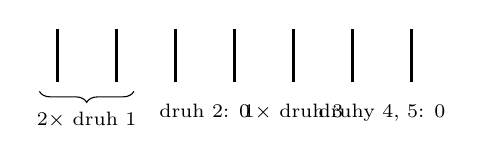
\begin{tikzpicture}[scale=0.75]
    \foreach \x/\t in {0/s, 1/s, 2/b, 3/b, 4/s, 5/b, 6/b} {
      \ifx\t s \node[colorofwisdom] at (\x,0) {\LARGE $\star$}; \else \draw[very thick] (\x,-0.45) -- (\x,0.45); \fi
    }
    \draw[decorate, decoration={brace, mirror, amplitude=4pt}] (-0.3,-0.6) -- (1.3,-0.6) node[midway, below=4pt, font=\scriptsize] {2$\times$ druh 1};
    \node[below, font=\scriptsize] at (2.5,-0.65) {druh 2: 0};
    \node[below, font=\scriptsize] at (4,-0.65) {1$\times$ druh 3};
    \node[below, font=\scriptsize] at (5.5,-0.65) {druhy 4, 5: 0};
  \end{tikzpicture}
\end{center}

\begin{problem}
  \begin{enumerate}[label=(\alph*)]
    \item Kolik je SPZ ve tvaru `číslice, písmeno, číslice, číslice, číslice, číslice, číslice', pokud máme $26$ písmen?
    \item Kolik různých slov (i nesmyslných) lze sestavit přeskládáním písmen slova BANANA?
    \item Kolika způsoby lze rozdělit $10$ stejných bonbonů mezi $4$ děti?
    \item Kolik je cest z levého dolního do pravého horního rohu mřížky $5\times 3$, pokud smíme chodit jen doprava a nahoru?
  \end{enumerate}
\end{problem}

\begin{solution}
  \begin{enumerate}[label=(\alph*)]
    \item $10\cdot 26\cdot 10^5 = 26\,000\,000$.
    \item $\frac{6!}{1!\,3!\,2!} = 60$.
    \item $\binom{4 + 10 - 1}{10} = \binom{13}{10} = \binom{13}{3} = 286$.
    \item Každá cesta je posloupnost $5$ kroků doprava a $3$ nahoru. Je to permutace s opakováním: $\frac{8!}{5!\,3!} = \binom{8}{3} = 56$. Červená cesta na obrázku odpovídá slovu PPNPNPPN (P = doprava, N = nahoru).
    \begin{center}
      \begin{tikzpicture}[scale=0.7]
        \draw[gray!50] (0,0) grid (5,3);
        \draw[ultra thick, colorofwisdom, ->] (0,0) -- (2,0) -- (2,1) -- (3,1) -- (3,2) -- (5,2) -- (5,3);
        \filldraw (0,0) circle (2pt) node[below left] {\small start};
        \filldraw (5,3) circle (2pt) node[above right] {\small cíl};
      \end{tikzpicture}
    \end{center}
  \end{enumerate}
\end{solution}

\section{Kombinační čísla a binomická věta}\label{sec:binomicka-veta}

\begin{definitionbox}
  \textbf{Vlastnosti kombinačních čísel}:
  \begin{enumerate}
    \item $\binom{n}{0} = \binom{n}{n} = 1$, $\binom{n}{1} = n$,
    \item $\binom{n}{k} = \binom{n}{n - k}$ \quad(souměrnost),
    \item $\binom{n}{k} + \binom{n}{k + 1} = \binom{n + 1}{k + 1}$ \quad(Pascalův vztah),
    \item $\binom{n}{0} + \binom{n}{1} + \cdots + \binom{n}{n} = 2^n$.
  \end{enumerate}

  \textbf{Binomická věta}: Pro všechna $a, b\in\mathbb{R}$ a $n\in\mathbb{N}$ platí
  \begin{equation*}
    {(a + b)}^n = \sum_{k=0}^{n}\binom{n}{k}a^{n-k}b^k = \binom{n}{0}a^n + \binom{n}{1}a^{n-1}b + \cdots + \binom{n}{n}b^n.
  \end{equation*}
\end{definitionbox}

Všechny vlastnosti se dají dokázat počítáním se vzorcem, ale mnohem hezčí jsou \textbf{kombinatorické důkazy}, kde stejnou věc spočítáme dvěma způsoby.

\begin{proof}[(vlastností 2--4 a binomické věty)]
  \textbf{Souměrnost}: Vybrat $k$ prvků, které \textit{vezmeme}, je totéž jako vybrat $n - k$ prvků, které \textit{nevezmeme}.

  \textbf{Pascalův vztah}: Kolika způsoby lze vybrat $k + 1$ prvků z $n + 1$? Označme jeden prvek jako `speciální'. Buď ho vybereme, a pak zbylých $k$ vybíráme z $n$ ostatních ($\binom{n}{k}$ způsobů), nebo ho nevybereme a všech $k + 1$ vybíráme z $n$ ostatních ($\binom{n}{k + 1}$ způsobů). Sečtením dostaneme $\binom{n + 1}{k + 1}$.

  \textbf{Součet řádku}: Levá strana počítá všechny podmnožiny $n$-prvkové množiny podle počtu prvků. Pravá strana počítá totéž jinak: u každého prvku se rozhodneme, zda ho vezmeme, nebo ne, což dává $2^n$ možností. Je to počet prvků potenční množiny z kapitoly 2.

  \textbf{Binomická věta}: Roznásobíme ${(a + b)}^n = (a + b)(a + b)\cdots(a + b)$. Z každé závorky vybereme buď $a$, nebo $b$. Člen $a^{n-k}b^k$ dostaneme, kdykoli vybereme $b$ z právě $k$ závorek. Těch závorek lze vybrat $\binom{n}{k}$ způsoby, a proto je to koeficient u $a^{n-k}b^k$.
\end{proof}

Pascalův vztah je přesně pravidlo, podle kterého se staví Pascalův trojúhelník z kapitoly~\ref{kap:vyrazy}: každé číslo je součtem dvou čísel nad ním. Čísla v $n$-tém řádku jsou $\binom{n}{0}, \binom{n}{1}, \ldots, \binom{n}{n}$. Tam jsme slíbili důkaz binomické věty a teď jsme ho dodali.
\begin{center}
  \begin{tikzpicture}[xscale=0.95, yscale=0.75]
    \foreach \n in {0,...,5} {
      \foreach \k in {0,...,\n} {
        \pgfmathtruncatemacro{\c}{round(factorial(\n)/(factorial(\k)*factorial(\n-\k)))}
        \node at ({\k - \n/2}, -\n) {\small $\c$};
      }
    }
    \draw[colorofwisdom, thick, rounded corners] (-0.85,-3.35) rectangle (0.85,-2.65);
    \draw[colorofwisdom, thick, ->] (-0.5,-3.35) -- (-0.1,-3.7);
    \draw[colorofwisdom, thick, ->] (0.5,-3.35) -- (0.1,-3.7);
    \draw[colorofwisdom, thick] (0,-4) circle (0.32);
    \node[right, font=\small, colorofwisdom] at (2.6,-3.4) {$\binom{3}{1} + \binom{3}{2} = \binom{4}{2}$, tedy $3 + 3 = 6$};
  \end{tikzpicture}
\end{center}

\begin{example}
  \begin{itemize}
    \item ${(x + 2)}^4 = x^4 + 4x^3\cdot 2 + 6x^2\cdot 4 + 4x\cdot 8 + 16 = x^4 + 8x^3 + 24x^2 + 32x + 16$.
    \item Koeficient u $x^3$ v ${(2x - 1)}^5$: člen je $\binom{5}{2}{(2x)}^3{(-1)}^2 = 10\cdot 8x^3 = 80x^3$.
    \item $1{,}01^{10} = {(1 + 0{,}01)}^{10}\approx 1 + 10\cdot 0{,}01 + 45\cdot 0{,}0001 = 1{,}1045$. Další členy jsou zanedbatelné (přesně $1{,}10462\ldots$). Takhle se počítalo před kalkulačkami.
  \end{itemize}
\end{example}

\begin{problem}
  \begin{enumerate}[label=(\alph*)]
    \item Vyřešte v $\mathbb{N}$: $\binom{n}{2} = 28$ a $\frac{(n + 1)!}{(n - 1)!} = 30$.
    \item Zjednodušte $\binom{n}{2} + \binom{n}{3}$.
    \item Určete člen, který neobsahuje $x$, v rozvoji ${\left(x + \frac{1}{x}\right)}^6$.
    \item Kolik podmnožin má množina $\{1, 2, \ldots, 10\}$? Kolik z nich má sudý počet prvků?
  \end{enumerate}
\end{problem}

\begin{solution}
  \begin{enumerate}[label=(\alph*)]
    \item $\frac{n(n - 1)}{2} = 28$, $n^2 - n - 56 = 0$, $n = 8$ (záporný kořen zahodíme). Dále $(n + 1)n = 30$, $n = 5$.
    \item Podle Pascalova vztahu $\binom{n + 1}{3}$.
    \item Obecný člen je $\binom{6}{k}x^{6-k}x^{-k} = \binom{6}{k}x^{6 - 2k}$. Bez $x$ pro $k = 3$: $\binom{6}{3} = 20$.
    \item $2^{10} = 1024$. Polovina z nich, tedy $512$, má sudý počet prvků. Z binomické věty pro $a = 1$, $b = -1$ totiž $0 = {(1 - 1)}^{10} = \binom{10}{0} - \binom{10}{1} + \binom{10}{2} - \cdots$, takže součet `sudých' kombinačních čísel je roven součtu `lichých'.
  \end{enumerate}
\end{solution}

\section{Odbočka --- Faktoriál z polovičky}

Faktoriál je definovaný jen pro přirozená čísla: $n!$ je počet způsobů, jak seřadit $n$ věcí. Co by mohlo znamenat $\left(\frac{1}{2}\right)!$? Seřadit půl věci? To nedává smysl. Ale matematici se nenechají odradit tím, že něco nedává smysl. V kapitole~\ref{kap:vyrazy} jsme takhle `nesmyslně' rozšířili mocniny na záporné a racionální exponenty, a pokaždé tak, aby dál platila stará pravidla. Pro faktoriál je to pravidlo $(n + 1)! = (n + 1)\cdot n!$.

Na obrázku vidíte body $[n, (n-1)!]$ pro $n = 1, 2, 3, 4$, tedy $1, 1, 2, 6$. Chceme jimi proložit hladkou křivku, která dál splňuje to rekurentní pravidlo. Takovou funkci v roce 1729 našel Leonhard Euler.

\begin{definitionbox}
  \textbf{Funkce gama}: Pro $x > 0$ definujeme
  \begin{equation*}
    \Gamma(x) = \int_0^{\infty} t^{x-1}e^{-t}\,\mathrm{d}t.
  \end{equation*}
  \textbf{Vlastnosti}:
  \begin{itemize}
    \item $\Gamma(x + 1) = x\,\Gamma(x)$ (stejné pravidlo jako u faktoriálu),
    \item $\Gamma(1) = 1$, a tedy $\Gamma(n + 1) = n!$ pro všechna $n\in\mathbb{N}_0$,
    \item $\Gamma\left(\frac{1}{2}\right) = \sqrt{\pi}$, a tedy `$\left(\frac{1}{2}\right)! = \Gamma\left(\frac{3}{2}\right) = \frac{\sqrt{\pi}}{2}\approx 0{,}886$'.
  \end{itemize}
\end{definitionbox}

\begin{proof}[(vztahu $\Gamma(x + 1) = x\Gamma(x)$)]
  Integrací per partes z kapitoly~\ref{kap:integraly} s $u = t^x$ a $v' = e^{-t}$:
  \begin{equation*}
    \Gamma(x + 1) = \int_0^{\infty}t^xe^{-t}\,\mathrm{d}t = {\big[-t^xe^{-t}\big]}_0^{\infty} + x\int_0^{\infty}t^{x-1}e^{-t}\,\mathrm{d}t = 0 + x\Gamma(x).
  \end{equation*}
  (Člen v hranaté závorce je nulový v nule i v nekonečnu, protože exponenciála $e^{-t}$ klesá rychleji, než jakákoli mocnina roste.) A $\Gamma(1) = \int_0^\infty e^{-t}\,\mathrm{d}t = 1$. Indukcí pak $\Gamma(n + 1) = n\Gamma(n) = \cdots = n!$.
\end{proof}

\begin{center}
  \begin{tikzpicture}[scale=0.85]
    \draw[->] (-2.3,0) -- (5,0) node[right] {\small $x$};
    \draw[->] (0,-5.4) -- (0,5.6) node[above] {\small $y$};
    \foreach \x in {-2,-1,1,2,3,4} \draw (\x,0.08) -- (\x,-0.08) node[below] {\tiny $\x$};
    \foreach \y in {-4,-2,2,4} \draw (0.08,\y) -- (-0.08,\y) node[left] {\tiny $\y$};
    \foreach \a in {0,-1,-2} \draw[dashed, gray] (\a,-5.3) -- (\a,5.4);
    \draw[thick, colorofwisdom] plot[smooth] coordinates {(0.200,4.591) (0.273,3.300) (0.347,2.572) (0.420,2.110) (0.493,1.796) (0.567,1.571) (0.640,1.404) (0.713,1.277) (0.787,1.180) (0.860,1.103) (0.933,1.043) (1.007,0.996) (1.080,0.960) (1.153,0.932) (1.227,0.912) (1.300,0.897) (1.373,0.889) (1.447,0.886) (1.520,0.887) (1.593,0.893) (1.667,0.903) (1.740,0.917) (1.813,0.935) (1.887,0.957) (1.960,0.984) (2.033,1.015) (2.107,1.050) (2.180,1.090) (2.253,1.135) (2.327,1.186) (2.400,1.242) (2.473,1.305) (2.547,1.374) (2.620,1.451) (2.693,1.537) (2.767,1.631) (2.840,1.734) (2.913,1.849) (2.987,1.976) (3.060,2.115) (3.133,2.270) (3.207,2.440) (3.280,2.629) (3.353,2.837) (3.427,3.068) (3.500,3.323) (3.573,3.607) (3.647,3.921) (3.720,4.269) (3.793,4.657) (3.867,5.088)};
    \draw[thick, colorofwisdom] plot[smooth] coordinates {(-0.770,-5.143) (-0.747,-4.800) (-0.725,-4.522) (-0.703,-4.296) (-0.680,-4.111) (-0.657,-3.961) (-0.635,-3.839) (-0.613,-3.741) (-0.590,-3.666) (-0.568,-3.610) (-0.545,-3.571) (-0.522,-3.550) (-0.500,-3.545) (-0.477,-3.556) (-0.455,-3.583) (-0.432,-3.627) (-0.410,-3.689) (-0.388,-3.771) (-0.365,-3.874) (-0.343,-4.002) (-0.320,-4.159) (-0.297,-4.350) (-0.275,-4.582) (-0.252,-4.866)};
    \draw[thick, colorofwisdom] plot[smooth] coordinates {(-1.883,4.839) (-1.860,4.181) (-1.837,3.715) (-1.815,3.370) (-1.792,3.108) (-1.770,2.905) (-1.748,2.747) (-1.725,2.622) (-1.702,2.523) (-1.680,2.447) (-1.657,2.390) (-1.635,2.348) (-1.613,2.320) (-1.590,2.306) (-1.567,2.303) (-1.545,2.312) (-1.522,2.332) (-1.500,2.363) (-1.478,2.407) (-1.455,2.463) (-1.433,2.532) (-1.410,2.616) (-1.388,2.718) (-1.365,2.838) (-1.343,2.981) (-1.320,3.151) (-1.297,3.353) (-1.275,3.594) (-1.252,3.885) (-1.230,4.241) (-1.208,4.681)};
    \foreach \x/\y in {1/1, 2/1, 3/2} \filldraw (\x,\y) circle (2.5pt);
    \filldraw (1.5,0.886) circle (2.5pt) node[below right, font=\tiny] {$\Gamma(\frac{3}{2}) = (\frac{1}{2})!$};
    \node[colorofwisdom, font=\small] at (3.4,4.9) {$y = \Gamma(x)$};
  \end{tikzpicture}
\end{center}

Černé body jsou obyčejné faktoriály $0! = 1! = 1$ a $2! = 2$ (bod $3! = 6$ v $x = 4$ už se do obrázku nevešel). Funkce gama mezi nimi vede hladce a vztah $\Gamma(x) = \frac{\Gamma(x + 1)}{x}$ ji rozšíří i na záporná čísla, kromě nuly a záporných celých čísel, kde má svislé asymptoty. Odtud mimochodem plyne další důvod, proč je $0! = 1$: je to prostě $\Gamma(1)$.

Že $\Gamma\left(\frac{1}{2}\right) = \sqrt{\pi}$, je jedna z těch matematických náhod, které nejsou náhodou. Po substituci $t = s^2$ se integrál změní na $\int_{-\infty}^{\infty}e^{-s^2}\,\mathrm{d}s$, tedy obsah pod Gaussovou křivkou, kterou uvidíme u normálního rozdělení v kapitole o pravděpodobnosti. A ten je roven $\sqrt{\pi}$. Kruh a pravděpodobnost se tu potkávají v jednom čísle.

\begin{note}
  Pro velká $n$ je faktoriál neprakticky velký, ale dá se dobře odhadnout \textbf{Stirlingovým vzorcem}
  \begin{equation*}
    n!\approx\sqrt{2\pi n}{\left(\frac{n}{e}\right)}^n.
  \end{equation*}
  Už pro $n = 10$ se liší jen o $0{,}8\,\%$ ($3\,598\,696$ místo $3\,628\,800$) a s rostoucím $n$ je relativní chyba čím dál menší. Ve vzorci jsou zase $\pi$ i $e$, přestože faktoriál je jen součin celých čísel.
\end{note}

\section{Odbočka --- Josephův problém}

Roku 67 našeho letopočtu obléhali Římané galilejské město Jotapata. Když město padlo, ukryl se židovský velitel Josephus se čtyřiceti svými muži v jeskyni. Muži se odmítli vzdát a rozhodli se raději zemřít. Podle Josephova vlastního vyprávění se domluvili, že se postaví do kruhu a budou se navzájem zabíjet podle losu, aby nikdo nemusel spáchat sebevraždu, kterou jejich víra zakazovala. Josephus a jeden další muž zůstali poslední, a místo aby splnili dohodu, vzdali se Římanům. Josephus pak přežil válku, stal se římským občanem a sepsal dějiny židovské války, ze kterých celý příběh známe.

Pozdější verze legendy (od matematiků, ne od historiků) z toho udělaly hádanku: $41$ lidí stojí v kruhu a počítá se dokola. Každý třetí je vyřazen, dokud nezůstane jediný. Na které místo se musí postavit Josephus, aby přežil? Odpověď je: na $31.$ místo, a jeho přítel na $16.$ místo, aby byli poslední dva.
\begin{center}
  \begin{tikzpicture}[scale=1.6]
    \foreach \i in {1,...,41} {
      \pgfmathsetmacro{\ang}{90-360*(\i-1)/41}
      \ifnum\i=31 \filldraw[colorofwisdom] (\ang:1) circle (2.2pt); \node[colorofwisdom, font=\scriptsize] at (\ang:1.22) {31};
      \else\ifnum\i=16 \filldraw[colorofwisdom] (\ang:1) circle (2.2pt); \node[colorofwisdom, font=\scriptsize] at (\ang:1.22) {16};
      \else \filldraw[black!40] (\ang:1) circle (1.2pt); \fi\fi
    }
    \node[font=\scriptsize] at (90:1.22) {1};
    \draw[->, gray] (80:0.75) arc (80:20:0.75);
    \node[font=\scriptsize, gray] at (0,0) {každý třetí ven};
  \end{tikzpicture}
\end{center}

Obecně, pokud vyřazujeme každého druhého z $n$ lidí, dá se poloha přeživšího spočítat přesně. Napíšeme $n = 2^m + l$, kde $2^m$ je největší mocnina dvojky nepřevyšující $n$ a $0\leq l < 2^m$. Přeživší stojí na místě $2l + 1$. Pro $41 = 32 + 9$ je to místo $19$. Zkuste si to ověřit na malém příkladu, například pro $n = 5$ (přežije třetí) nebo $n = 8$ (přežije první). Úloha se dnes používá jako klasické cvičení v programování, kde se jí říká \textit{Josephus problem}. Je to asi jediná programovací úloha, jejímž historickým základem je hromadná sebevražda v jeskyni.

\section{Shrnutí a otázky k ústní zkoušce}

\begin{problem}
  Odpovězte vlastními slovy:
  \begin{enumerate}
    \item Vysvětlete pravidlo součtu a součinu. Jak souvisí s množinami?
    \item Co je faktoriál? Proč je $0! = 1$?
    \item Co jsou variace, permutace a kombinace bez opakování? Odvoďte vzorce pro jejich počet.
    \item Jak poznáte, který typ výběru v úloze použít?
    \item Co jsou variace, permutace a kombinace s opakováním? Vysvětlete vzorec pro permutace s opakováním.
    \item Jaké vlastnosti mají kombinační čísla? Dokažte Pascalův vztah.
    \item Vyslovte a dokažte binomickou větu. Jak souvisí s Pascalovým trojúhelníkem?
    \item Kolik podmnožin má $n$-prvková množina a proč?
  \end{enumerate}
\end{problem}
